
\begin{figure}[h]
        \centering
        \begin{subfigure}[b]{0.300\textwidth}
            \centering
            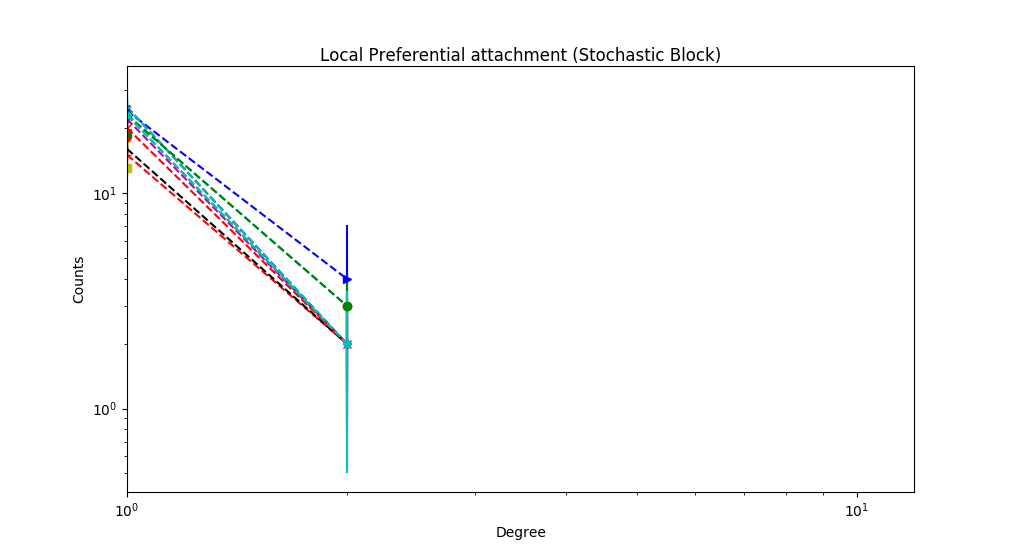
\includegraphics[width=\textwidth]{img/expe/1_mmsb/figure_2}
            \label{fig:mean and std of net14}
            \caption {{\small Network1}}    
        \end{subfigure}
        \begin{subfigure}[b]{0.300\textwidth}
            \centering
            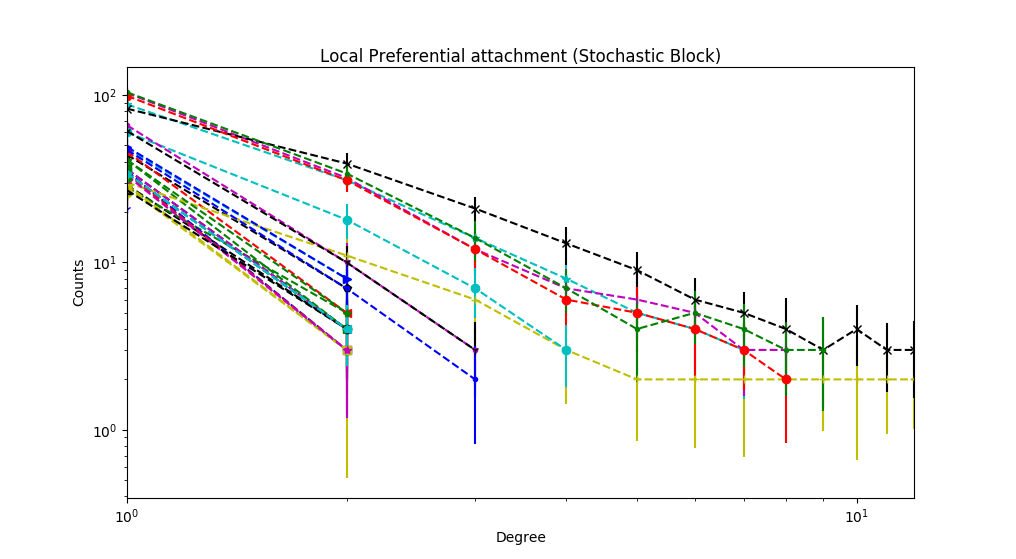
\includegraphics[width=\textwidth]{img/expe/2_mmsb/figure_2}
            \label{fig:mean and std of net14}
            \caption {{\small Network2}}    
        \end{subfigure}
        \begin{subfigure}[b]{0.300\textwidth}
            \centering
            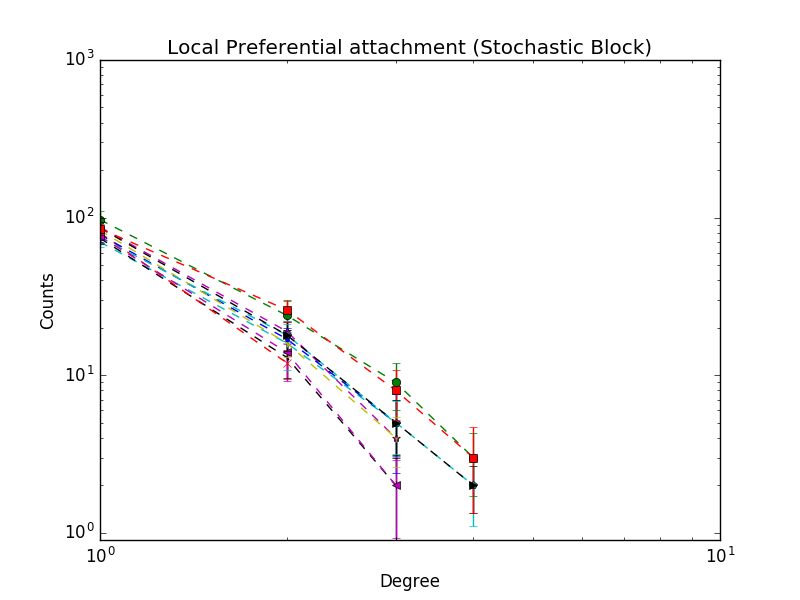
\includegraphics[width=\textwidth]{img/expe/3_mmsb/figure_2}
            \label{fig:mean and std of net14}
            \caption {{\small Network3}}    
        \end{subfigure}
        \begin{subfigure}[b]{0.300\textwidth}
            \centering
            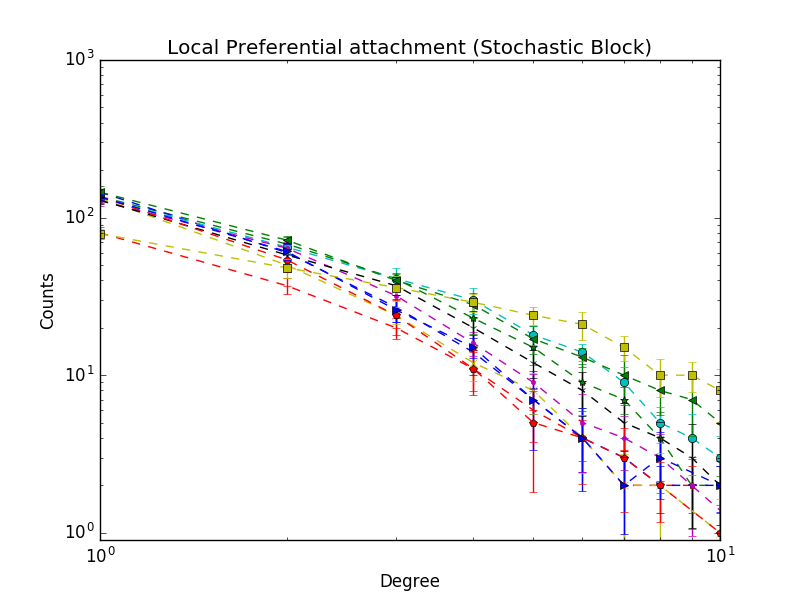
\includegraphics[width=\textwidth]{img/expe/4_mmsb/figure_2}
            \label{fig:mean and std of net14}
            \caption {{\small Network4}}    
        \end{subfigure}
        \begin{subfigure}[b]{0.300\textwidth}
            \centering
            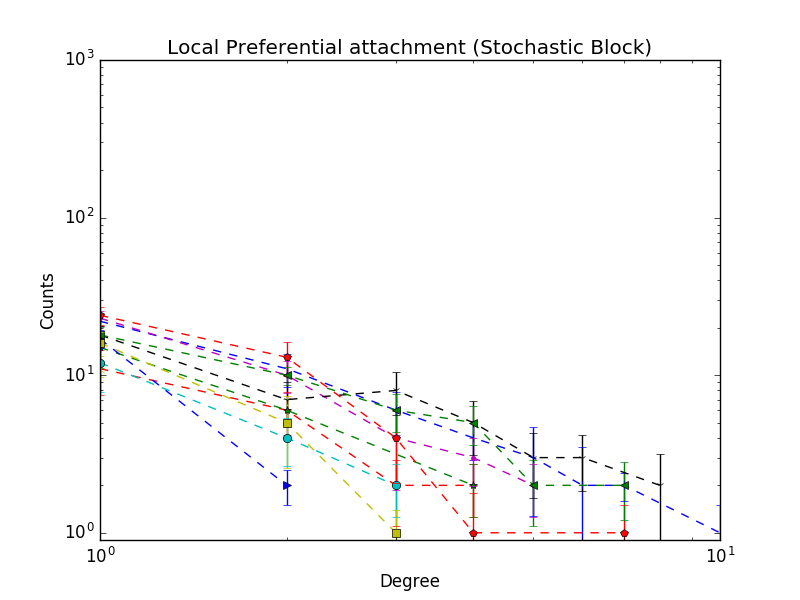
\includegraphics[width=\textwidth]{img/expe/5_mmsb/figure_2}
            \label{fig:mean and std of net14}
            \caption {{\small Manufacturing}}    
        \end{subfigure}
        \begin{subfigure}[b]{0.300\textwidth}
            \centering
            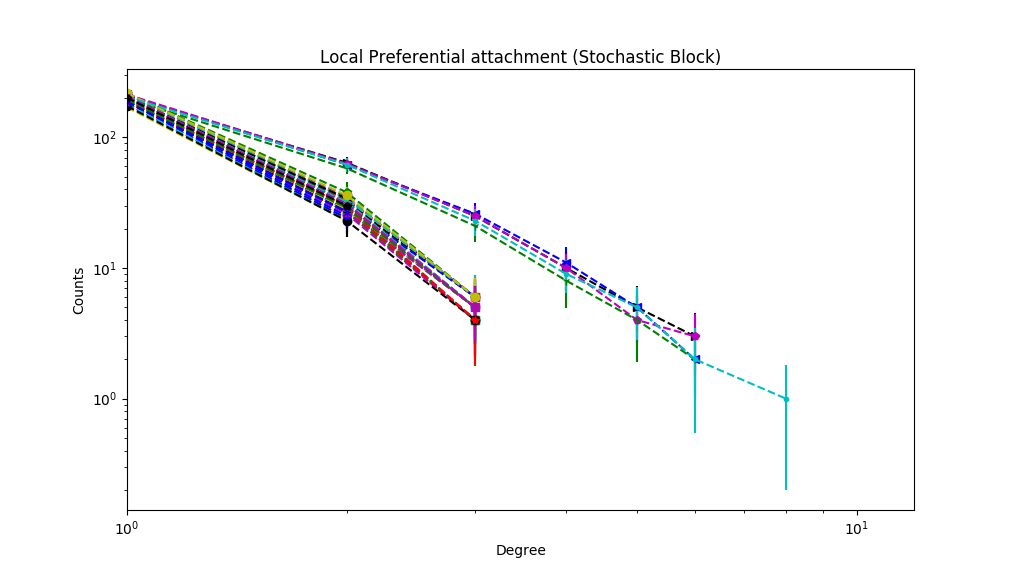
\includegraphics[width=\textwidth]{img/expe/6_mmsb/figure_2}
            \caption {{\small UC Irvine}}    
            \label{fig:mean and std of net14}
        \end{subfigure}
        %\quad
        %\hfill
        \caption{IMMSB Local degree distribution in the $M_e$ settings. } 
\end{figure}
